\chapter{火球、參考系與四維向量}

我們先從高能碰撞討論中留下的一個問題談起。兩個重原子核碰撞後形成的，是一個劇烈變化的物體，而非寧靜的天文黑洞。那麼，用視界描述這種碰撞究竟有何意義？答案會帶我們先認識強耦合物質的五維圖像，再探討一系列加速器的實際問題，最後回到狹義相對論的幾何。到最後，速度和動量都成了四維向量，而能量也與動量的三個分量並列。

\section{第五維中的火球}

\begin{classroomqa}
\audiencequestion{碰撞產生的物體並不穩定，形狀也會改變。這樣複雜的物體怎麼能稱為黑洞？}
\lecturerresponse{想像第五個空間方向延伸於地板和天花板之間。該方向上的引力會把激發態拉向地板。碰撞在那裡沉積了一團高熱能量；它會擴散、改變形狀，卻仍可具有視界、溫度和熵。}
\end{classroomqa}

想像粒子，或者更形象地說，小弦，在這個五維世界中運動。落向地板的激發態，在四維中呈現為強子：質子、中子、介子，以及其他延展的複合物體。附著在天花板附近的激發態則呈現得較為基本。因此，垂直位置是一種以幾何方式編碼尺度的手段：地板代表長距離的強子區域，天花板則代表短距離的自由度。

兩個強子碰撞時，地板附近的兩個物體相撞，激起大量能量。產物不是剛體，而是一團帶有視界的高熱物質，彷彿五維引力場中的一灘水。它既不是普通四維空間中的天文黑洞，也不是附著在天花板上的普朗克尺度黑洞，而是地板附近強作用火球的引力描述。

在高能下，入射原子核會因洛倫茲收縮而變成薄薄的煎餅狀。它們碰撞後，將能量沉積在一小塊區域，並產生逐漸趨近平衡的流體。夸克--膠子電漿的小黏滯性，是它令人驚訝的特徵之一。在五維描述中，同樣的演化就是扭曲視界的弛豫。

\begin{figure}[H]
\centering
\includegraphics[width=0.82\textwidth]{lecture_05_figure_01.png}
\caption{第五維的地板與天花板圖像。碰撞後，中央這團帶有視界的物質沿著地板擴散。}
\lectureframe{00:04:22}
\end{figure}

視界不會永遠存在。霍金輻射會帶走能量；在四維描述中，這些輻射就是碰撞後湧現的一簇簇普通強子。用這種語言來說，探測器事件中的數千條徑跡，就是從對偶黑洞中蒸發出來的粒子。

\subsection{額外維度是真實存在的嗎？}

\begin{classroomqa}
\audiencequestion{第五維是空間維度嗎？圖中地板與天花板之間的那條線，真的是沿著這個方向延伸嗎？}
\lecturerresponse{是的。這是類空方向，而在該五維幾何中畫出的曲面就是視界。至於額外方向是否``真實存在''，或者只是等價的數學描述，則是更深一層的問題。}
\end{classroomqa}

有用的說法不是引力取代了量子色動力學，而是兩種語言可能描述同一套物理。在四維語言中，這是一團由夸克和膠子組成的高熱火球，沒有通常意義下的引力場。在五維語言中，則有引力和視界。如果這種對應成立，那麼只要兩種計算都做得到，嚴謹的 QCD 計算就必須和對偶的引力計算一致。

\begin{classroomqa}
\audiencequestion{QCD 中既沒有引力，也沒有視界。黑洞圖像是在加入新物理，還是只用另一種方式描述火球？}
\lecturerresponse{在四維中，它是夸克和膠子組成的電漿；在五維版本中，則有帶視界的引力描述。這種描述的優勢在於計算。強耦合 QCD 極難計算，但某些視界性質---尤其是黏滯性---相對容易計算。}
\end{classroomqa}

``真實維度''和``數學類比''之間的區別，不必先有定論，這種描述才有用。當某個結構能把其他變數整合成一組更簡潔、更連貫的定律時，它便具有物理解釋的價值。儘管如此，也不應誇大其意義：規範／引力對偶性應用於觀測到的夸克--膠子電漿時，提供的是強耦合動力學的模型，並不能證明現實世界的 QCD 已知具有精確的引力對偶。\editorialnote{這項限定明確說明了 QCD 應用在現代物理中的定位；它不會改變此處闡述的五維機制。}

\section{為什麼對撞機要讓束流互撞}

現在來看幾個實際問題：為什麼要讓兩束運動中的粒子束互撞，而不是讓一束粒子撞上靜止靶？為什麼環形加速器這麼大？為什麼電子和質子的處理方式不同？這些問題都與相對論能量有關。

\begin{classroomqa}
\audiencequestion{為什麼要讓兩束粒子束互撞，而不是用一束高能粒子束撞擊靜止靶？}
\lecturerresponse{產生新粒子所需的能量，取決於質心系中可用的能量。兩束能量相等、方向相反的相對論性粒子束，總動量為零，因此幾乎所有能量都可用於碰撞。若靶固定，入射能量中有很大一部分只能成為質心的運動。}
\end{classroomqa}

對於兩個動量大小為\(p\)、方向相反的超相對論性粒子，在\(c=1\)單位下，講義中的估算為
\begin{equation}
E_{\mathrm{cm}}^{\mathrm{collider}}\simeq 2p.
\end{equation}
固定靶的相應估算則只隨束流動量的平方根增加，
\begin{equation}
E_{\mathrm{cm}}^{\mathrm{fixed}}\sim \sqrt{mp}.
\end{equation}
關鍵在於標度關係，而非省略的數值因子：束流能量加倍，對撞機的質心能量也加倍；固定靶的質心能量則只增加為原來的平方根倍。

用不變量計算，可以精確比較兩者。若\(P_1\)和\(P_2\)是入射四維動量，則
\begin{equation}
s=(P_1+P_2)^2,
\qquad E_{\mathrm{cm}}=\sqrt{s}.
\end{equation}
對於能量為\(E\)、等能量且反向傳播的兩束粒子，空間動量彼此抵消，因此\(\sqrt{s}=2E\)。若能量為\(E\gg m\)的入射粒子撞上靜止的等質量靶，則
\begin{equation}
s=2m^2+2mE,
\qquad
\sqrt{s}\simeq \sqrt{2mE}
\qquad (c=1).
\end{equation}
這個簡短的不變量推導補上了口頭估算中省略的因子。\editorialnote{列出這項推導，是為了讓講義中的標度論證可以重現。}

\begin{classroomqa}
\audiencequestion{環形加速器非得這麼大不可，有什麼根本原因嗎？能不能讓同一束粒子多繞幾圈，通過較小的機器？}
\lecturerresponse{磁場和材料都會形成限制。粒子每公尺所能增加的能量有限，因此能量更高的機器需要更長的有效加速距離。環越小，所需的橫向加速度也越大；而帶電粒子在加速時會輻射。環太小時，束流輻射掉能量的速度就會和機器供應能量的速度一樣快。}
\end{classroomqa}

偏轉關係近似為
\begin{equation}
p=qBR,
\end{equation}
因此，在磁場\(B\)固定時，動量\(p\)越大，所需半徑\(R\)也越大。提高束流能量的工作由射頻腔完成；磁鐵則負責使束流偏轉並聚焦。大致來說，黑板上的結論仍然成立：場強和輻射損失使我們無法把任意高能的加速器塞進小環裡。

即使速率不變，圓周運動仍有加速度，因為速度方向持續改變。加速中的電荷會發射同步輻射。直線加速器沒有持續轉向所造成的損失，但短暫的加速推進本身也並非完全沒有輻射。環形加速器接受轉向帶來的代價，換取每一圈都能重複使用同一套設備。

\begin{classroomqa}
\audiencequestion{為什麼電子會和 SLAC 的直線加速器相聯，而環形高能對撞機卻使用質子或其他強子？}
\lecturerresponse{電子的質量小得多。在相同的高能量下，電子的洛倫茲因子大得多；環形加速會使它們發出強得多的輻射。較重的質子可以在環中反覆運行，每經過一次就增加一些能量，直到同步輻射損失變得難以承受。}
\end{classroomqa}

在能量和環半徑固定時，輻射功率對粒子質量的依賴非常陡峭，
\begin{equation}
P_{\mathrm{sync}}\propto \frac{E^4}{m^4R^2}.
\end{equation}
因此，電子--質子的差異，遠比``較輕的粒子跑得比較快''這句話所暗示的更大得多：兩束粒子的速度都可能已非常接近\(c\)，但它們的洛倫茲因子和輻射損失卻大不相同。\editorialnote{偏轉關係和同步輻射的標度律，讓講義中的加速器定性論證有了精確的表述；這些推導並未在黑板上完成。}

\begin{classroomqa}
\audiencequestion{為什麼不也用直線加速器加速強子？}
\lecturerresponse{可以。難處在於所需長度。在環形加速器中，同一粒子會多次通過加速結構；要達到相同效果，直線強子加速器就得長得驚人。實用的折衷方案是採用大型環形加速器，讓環大到質子輻射仍在可容忍範圍內。}
\end{classroomqa}

這些加速器問題正好說明，為什麼牛頓力學的規則不敷使用。現在我們回到狹義相對論，建立一套能有系統地比較這些情況的語言。

\section{車庫與加長型禮車}

想像一座約十二英尺長的車庫，以及一輛約二十英尺長的加長型禮車。司機不斷加速，直到禮車因洛倫茲收縮而變短，希望它能塞進車庫。在車庫參考系中，運動中的禮車較短，因此看起來塞得進去。然而在禮車參考系中，運動中的車庫較短，因此看起來塞不進去。整輛禮車到底能不能完全在車庫裡？

把兩扇門都打開，免得撞上牆壁的問題分散我們的注意力。說禮車在車庫裡，意思是它的車頭和車尾\emph{同時}都在車庫內。整個謎題的關鍵就在「同時」這個詞。

畫一張時空圖，讓\(t\)軸垂直、\(x\)軸水平。在\(c=1\)單位下，光線形成\(45^\circ\)光錐。車庫靜止，因此兩扇門的世界線是垂直線。禮車的車頭和車尾則沿著兩條平行斜線運動。運動參考系的\(t'\)軸朝光錐方向傾斜，而其同時線平行於傾斜的\(x'\)軸。

\begin{figure}[H]
\centering
\includegraphics[width=0.82\textwidth]{lecture_05_figure_02.png}
\caption{完整的車庫--禮車時空圖。垂直線標示車庫的邊界；斜線描繪禮車的兩端。水平和傾斜的截線，分別代表兩個參考系不同的同時性切面。}
\lectureframe{00:31:05}
\end{figure}

在車庫參考系中，一條水平線可以在兩條車庫門的世界線之間，穿過禮車兩端的世界線。在車庫的那個時刻，車尾已進入車庫，車頭還沒出去。收縮後的禮車整輛都在車庫內。

在禮車參考系中，相關的同時事件位於一條斜線上。從車尾進入車庫的事件畫出這條線；線與車頭世界線相交時，車頭早已通過遠端的門。依照禮車自身的同時性，整輛禮車從未完全位於車庫內。兩種說法都成立，因為各自比較的是不同的一對事件。

\begin{classroomqa}
\audiencequestion{兩條綠色世界線和它們之間的水平線段構成平行四邊形嗎？那條黑色線段就是車輛的長度嗎？}
\lecturerresponse{水平線段代表洛倫茲收縮後的長度，因為它的兩個端點在車庫參考系中同時。固有長度則由禮車參考系中同時的兩個端點決定，這兩點位於平行於\(x'\)的直線上。兩種測量是在同一對世界線上取不同的截線。}
\end{classroomqa}

若固有長度為\(L_0\)，車庫參考系中的水平截線長度就是\begin{equation}
L=\frac{L_0}{\gamma},
\qquad
\gamma=\frac{1}{\sqrt{1-v^2/c^2}}.
\end{equation}
單靠公式無法解開這個悖論；圖可以，因為圖顯示了比較的是哪些事件。每當相對論的問題似乎導出兩個互不相容的答案，就要留意其中是否暗中用到了「``同時''」這個概念。

\section{四個座標與兩種指標位置}

要從謎題轉向運動定律，我們需要一套能反映幾何的記號。把座標寫成
\begin{equation}
(X^1,X^2,X^3,X^0)=(x,y,z,t),
\qquad X^\mu=(x,y,z,t),
\end{equation}
其中，\(\mu\)依序取\(1,2,3,0\)。這個排列把時間放在書寫順序的最後，儘管它的指標是\(0\)，與黑板上採用的慣例相同。

\begin{classroomqa}
\audiencequestion{我們是令\(c=1\)嗎？如果恢復一般單位，時間座標是不是應該寫成\(ct\)？}
\lecturerresponse{是的。在建立幾何時，我們令\(c=1\)；遇到量綱或非相對論極限等問題時，再把\(c\)的因子放回去。使用慣常的長度單位時，時間座標是\(ct\)。}
\end{classroomqa}

同一個向量也可以用下指標表示。採用這裡的符號約定，
\begin{equation}
X_\mu=(-x,-y,-z,t).
\end{equation}
因此，降低指標會使三個空間分量的符號反轉，而時間分量的符號不變。例如，
\begin{equation}
X^\mu=(3,2,4,10)
\quad\Longrightarrow\quad
X_\mu=(-3,-2,-4,10).
\end{equation}
這不是兩個時空點，而是同一個幾何物體的兩種分量表示法。

\begin{classroomqa}
\audiencequestion{哪些分量是協變、哪些是逆變？標記應該寫成上標還是下標？}
\lecturerresponse{上指標分量是逆變的；下指標分量是協變的。課堂上有個好記的口訣：``co 在下，contra 在上。''物理學家也常直接說「上面」和「下面」。}
\end{classroomqa}

這套記號的優點，在不變縮併中一目了然：
\begin{equation}
X_\mu X^\mu=t^2-x^2-y^2-z^2.
\label{eq:l5-interval}
\end{equation}
用微分表示，就是
\begin{equation}
d\tau^2=dt^2-dx^2-dy^2-dz^2
\qquad (c=1).
\label{eq:l5-proper-time}
\end{equation}
對於類時運動，\(d\tau\)是沿著世界線運動的時鐘所記錄的時間。

同一個指標若在上方出現一次、下方出現一次，就表示要對該指標求和。愛因斯坦求和慣例將
\begin{equation}
\sum_{\mu}X_\mu X^\mu
\end{equation}
簡寫成式~\eqref{eq:l5-interval}中的形式。這不只是節省排版空間，也免去了在每個方程中手動重寫閔可夫斯基幾何交錯的正負號。

\begin{classroomqa}
\audiencequestion{\(\tau\)是固有時的標準符號嗎？}
\lecturerresponse{是的。有時也會用符號\(s\)，但\(\tau\)是表示固有時的標準選擇。}
\end{classroomqa}

\section{作為簡單對稱操作的旋轉}

洛倫茲推移會混合空間和時間。在研究那個矩陣之前，先來看較熟悉的操作：旋轉空間座標軸。如果相對運動方向不固定在某個軸上，我們可以先旋轉座標軸，讓該方向成為新的\(x\)軸，再施加已知的洛倫茲推移。因此，旋轉是構造的一部分，並非多餘的插曲。

繞\(z\)軸旋轉角度\(\theta\)時，
\begin{align}
x'&=x\cos\theta+y\sin\theta,\nonumber\\
y'&=-x\sin\theta+y\cos\theta,\label{eq:l5-rotation}\\
z'&=z.\nonumber
\end{align}
在\(\theta=0\)時，這些方程會給出\(x'=x\)和\(y'=y\)；在\(\theta=\pi/2\)時，則會以預期的符號互換兩個座標軸。

此變換會保持歐幾里得距離不變。令
\(c_\theta=\cos\theta\)和\(s_\theta=\sin\theta\)，則
\begin{align}
x'^2+y'^2
&=(xc_\theta+ys_\theta)^2+(-xs_\theta+yc_\theta)^2\nonumber\\
&=x^2(c_\theta^2+s_\theta^2)
  +y^2(s_\theta^2+c_\theta^2)\nonumber\\
&\quad+2xyc_\theta s_\theta-2xyc_\theta s_\theta\nonumber\\
&=x^2+y^2.
\end{align}
交叉項相消，因此\(c_\theta^2+s_\theta^2=1\)。又因為\(z'=z\)，整個長度\(x^2+y^2+z^2\)也保持不變。

同一組方程也可以寫成一個矩陣方程：
\begin{equation}
\begin{pmatrix}x'\\y'\\z'\end{pmatrix}
=
\underbrace{\begin{pmatrix}
\cos\theta&\sin\theta&0\\
-\sin\theta&\cos\theta&0\\
0&0&1
\end{pmatrix}}_{M}
\begin{pmatrix}x\\y\\z\end{pmatrix}.
\label{eq:l5-rotation-matrix}
\end{equation}
用指標記號表示則為
\begin{equation}
x'^i=M^i{}_{j}x^j,
\qquad i,j=1,2,3.
\end{equation}

\begin{figure}[H]
\centering
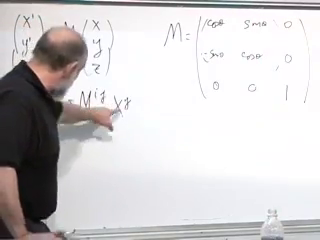
\includegraphics[width=0.82\textwidth]{lecture_05_figure_03.png}
\caption{空間旋轉的矩陣方程及其指標記號表示法。}
\lectureframe{01:00:40}
\end{figure}

\section{洛倫茲矩陣與速度合成}

沿\(x\)方向運動時，在\(c=1\)單位下，洛倫茲變換為
\begin{align}
x'&=\gamma_v(x-vt), & y'&=y,\nonumber\\
z'&=z, & t'&=\gamma_v(t-vx),
\end{align}
其中
\begin{equation}
\gamma_v=\frac{1}{\sqrt{1-v^2}}.
\end{equation}
若分量順序採用\((x,y,z,t)\)，則可寫成
\begin{equation}
\begin{pmatrix}x'\\y'\\z'\\t'\end{pmatrix}
=
\begin{pmatrix}
\gamma_v&0&0&-\gamma_vv\\
0&1&0&0\\
0&0&1&0\\
-\gamma_vv&0&0&\gamma_v
\end{pmatrix}
\begin{pmatrix}x\\y\\z\\t\end{pmatrix}.
\label{eq:l5-lorentz-matrix}
\end{equation}

\begin{figure}[H]
\centering
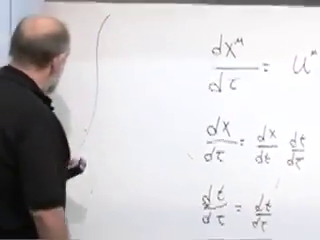
\includegraphics[width=0.82\textwidth]{lecture_05_figure_04.png}
\caption{\(4\times4\)洛倫茲矩陣。只有\(x\)和\(t\)分量會混合；\(y\)和\(z\)則保持不變。}
\lectureframe{01:04:40}
\end{figure}

矩陣乘法現在可以回答一個物理問題。假設有位觀察者以速度\(v\)相對於我們運動，另一位觀察者再以速度\(u\)相對於前一位觀察者運動，而且都沿同一軸。牛頓運動學會給出\(w=u+v\)，這樣一來，兩個\(3c/4\)的速度就可能合成為\(3c/2\)。相對論必須給出不同的規則。

洛倫茲推移中起作用的部分是\(2\times2\)矩陣：
\begin{equation}
B(v)=\gamma_v
\begin{pmatrix}1&-v\\-v&1\end{pmatrix}.
\end{equation}
將兩個推移複合，得到
\begin{align}
B(u)B(v)
&=\gamma_u\gamma_v
\begin{pmatrix}1&-u\\-u&1\end{pmatrix}
\begin{pmatrix}1&-v\\-v&1\end{pmatrix}\nonumber\\
&=\gamma_u\gamma_v
\begin{pmatrix}
1+uv&-(u+v)\\
-(u+v)&1+uv
\end{pmatrix}.
\label{eq:l5-composed-boost}
\end{align}
非對角元素與對角元素的比值，可用來求出合成推移的速度：
\begin{equation}
w=\frac{u+v}{1+uv}
\qquad(c=1).
\end{equation}
恢復量綱後，
\begin{equation}
w=\frac{u+v}{1+uv/c^2}.
\label{eq:l5-velocity-addition}
\end{equation}

\begin{figure}[H]
\centering
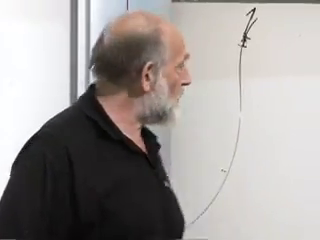
\includegraphics[width=0.82\textwidth]{lecture_05_figure_05.png}
\caption{複合推移的矩陣，以及自然單位下的速度\(w=(u+v)/(1+uv)\)。}
\lectureframe{01:15:35}
\end{figure}

若\(u\)和\(v\)都接近\(c\)，分子就趨近\(2c\)，分母則趨近\(2\)，所以\(w\)會趨近\(c\)，而非\(2c\)。更一般地說，式~\eqref{eq:l5-velocity-addition}會把亞光速輸入映成亞光速結果。矩陣乘法自動保證了速度上限。

\section{四維向量與普通速度為何不適用}

四維向量是指一種物體，其四個分量在旋轉和洛倫茲推移下的變換方式，與時空座標相同。若\(V^\mu\)是四維向量，依照我們的符號約定，
\begin{equation}
V_\mu=(-V^1,-V^2,-V^3,V^0),
\end{equation}
它的不變範數為
\begin{equation}
V_\mu V^\mu=(V^0)^2-(V^1)^2-(V^2)^2-(V^3)^2.
\end{equation}
對於兩個四維向量\(V^\mu\)和\(W^\mu\)，縮併
\begin{equation}
W_\mu V^\mu
=W^0V^0-W^1V^1-W^2V^2-W^3V^3
\end{equation}
也同樣是不變量。分量會隨參考系改變，縮併則不會。

普通速度只有三個分量：
\begin{equation}
\mathbf v=\left(\frac{dx}{dt},\frac{dy}{dt},\frac{dz}{dt}\right).
\end{equation}
光是附上\(dt/dt=1\)，並不能讓它成為有用的四維向量。如此一來，第四個分量只是平凡的數值，整個物體也不會依照洛倫茲變換作線性變換。座標時間\(t\)會因參考系而異，因此對\(t\)微分會破壞所需的變換律。

用固有時就能解決這個問題。沿著世界線定義
\begin{equation}
u^\mu=\frac{dX^\mu}{d\tau}.
\label{eq:l5-four-velocity}
\end{equation}
微分\(dX^\mu\)是四維向量，而\(d\tau\)是不變量，因此兩者之比也是四維向量。``固有''這個形容詞，指的是分母中的時鐘。

鏈鎖律將這個物體與普通速度連結起來：
\begin{equation}
\frac{dx}{d\tau}=\frac{dx}{dt}\frac{dt}{d\tau},
\end{equation}
對\(y\)和\(z\)也一樣。由式~\eqref{eq:l5-proper-time}可得
\begin{align}
\left(\frac{d\tau}{dt}\right)^2
&=1-\left(\frac{dx}{dt}\right)^2
    -\left(\frac{dy}{dt}\right)^2
    -\left(\frac{dz}{dt}\right)^2\nonumber\\
&=1-v^2
\qquad(c=1),
\end{align}
因此
\begin{equation}
\frac{dt}{d\tau}=\gamma_v=\frac{1}{\sqrt{1-v^2}}.
\end{equation}
四個分量為
\begin{equation}
u^i=\gamma_v v^i,
\qquad
u^0=\gamma_v
\qquad(c=1).
\label{eq:l5-four-velocity-components}
\end{equation}
在低速下，\(u^i\simeq v^i\)且\(u^0\simeq1\)。接近光速時，\(\gamma_v\)會無界增大，固有速度也就與普通速度大不相同。

\begin{figure}[H]
\centering
\includegraphics[width=0.82\textwidth]{lecture_05_figure_06.png}
\caption{以普通速度和洛倫茲因子表示的固有速度四個分量。}
\lectureframe{01:34:40}
\end{figure}

恢復慣用單位並使用\(X^0=ct\)，即可得到標準形式
\begin{equation}
U^\mu=(\gamma_v\mathbf v,\gamma_v c)
\end{equation}
這裡採用空間分量在前的排列順序。其不變範數為
\begin{equation}
U_\mu U^\mu=c^2.
\end{equation}
因此，所有有質量粒子的四維速度都具有相同的不變大小，儘管各自的空間速度會隨參考系而異。

\section{世界線的切向量}

式~\eqref{eq:l5-four-velocity}可以用一個熟悉的歐幾里得模型來理解。沿著普通三維空間中的一條曲線，
\begin{equation}
ds^2=dx^2+dy^2+dz^2.
\end{equation}
微分位移\((dx,dy,dz)\)沿著曲線方向，但不是單位向量。以弧長相除後得到
\begin{equation}
\mathbf T=
\left(\frac{dx}{ds},\frac{dy}{ds},\frac{dz}{ds}\right),
\qquad
\mathbf T\cdot\mathbf T=1.
\end{equation}
相對論中的構造概念相同，只是以固有時取代歐幾里得弧長。向量\(u^\mu=dX^\mu/d\tau\)與世界線相切。

\begin{figure}[H]
\centering
\includegraphics[width=0.82\textwidth]{lecture_05_figure_07.png}
\caption{歐幾里得空間中的切向量構造：將微分位移除以弧長微元\(ds\)。固有時沿類時世界線扮演相同的角色。}
\lectureframe{01:39:30}
\end{figure}

\begin{classroomqa}
\audiencequestion{若\(c=1\)，固有時和固有距離就是同一回事嗎？}
\lecturerresponse{令\(c=1\)，只是讓時間和距離使用相同單位，並不會消去時空幾何中的負號。在歐幾里得類比中，\(s\)是沿空間曲線測量的普通距離；沿著類時世界線，\(\tau\)則是時鐘測得的經過時間。兩種構造相似，但幾何並不相同。}
\end{classroomqa}

再微分一次，便定義出固有加速度：
\begin{equation}
a^\mu=\frac{du^\mu}{d\tau}.
\end{equation}
在相對論化的牛頓第二定律中，必須以這個量取代\(d^2\mathbf x/dt^2\)。由於\(u_\mu u^\mu\)為常數，
\begin{equation}
\frac{d}{d\tau}(u_\mu u^\mu)=2u_\mu a^\mu=0,
\end{equation}
因此四維加速度與四維速度在閔可夫斯基幾何下互相正交。\editorialnote{這個正交關係由不變範數立即可得，也是該定義接下來的一項數學推論。}

\section{四維動量與能量}

動量是最後一個例子，因為它在碰撞和衰變中守恆。粒子的內禀質量\(m\)固定不變，通常稱為靜止質量，不會隨速度改變。相對論動量是這個固定質量乘上四維速度：
\begin{equation}
p^\mu=mu^\mu.
\label{eq:l5-four-momentum}
\end{equation}
在\(c=1\)單位下，
\begin{equation}
p^i=\gamma_v m v^i,
\qquad
p^0=\gamma_v m.
\end{equation}
低速時\(\gamma_v\simeq1\)，所以空間分量會還原為牛頓動量\(m\mathbf v\)。高速時，這些分量的增長速度則超過\(m\mathbf v\)。

時間分量就是能量。採用慣用單位並使用\(X^0=ct\)，
\begin{equation}
P^\mu=(\mathbf p,E/c)
=(\gamma_v m\mathbf v,\gamma_v mc),
\end{equation}
因此
\begin{equation}
E=\gamma_v mc^2
=mc^2\left(1-\frac{v^2}{c^2}\right)^{-1/2}.
\label{eq:l5-relativistic-energy}
\end{equation}

要還原普通力學，令
\(\epsilon=v^2/c^2\ll1\)。利用二項式展開可得
\begin{equation}
(1-\epsilon)^p=1-p\epsilon+O(\epsilon^2).
\end{equation}
取\(p=-1/2\)，則
\begin{align}
E
&=mc^2\left(1-\frac{v^2}{c^2}\right)^{-1/2}\nonumber\\
&=mc^2\left[1+\frac12\frac{v^2}{c^2}
  +O\!\left(\frac{v^4}{c^4}\right)\right]\nonumber\\
&=mc^2+\frac12mv^2+O\!\left(\frac{mv^4}{c^2}\right).
\label{eq:l5-energy-expansion}
\end{align}

\begin{figure}[H]
\centering
\includegraphics[width=0.82\textwidth]{lecture_05_figure_08.png}
\caption{相對論能量的低速展開，顯示出靜止能量和牛頓力學中的動能。}
\lectureframe{01:51:30}
\end{figure}

第一項\(mc^2\)即使粒子靜止時也存在。在牛頓力學中，若粒子集合固定且各粒子的質量不變，這一項在運動前後都加上同一個常數，所以熟悉的能量計算只需考慮\(\tfrac12mv^2\)。相對論則揭示，被忽略的常數其實一直都代表物理能量。

因此，能量和動量不是彼此無關的守恆定律，而是同一個守恆四維向量的四個分量。洛倫茲推移會將兩者混合：一位觀察者所說的能量，有一部分會成為另一位觀察者所說的動量，反過來也一樣。儘管如此，對孤立系統而言，在任何慣性參考系中，總四維動量在每次碰撞或衰變前後都相同。

這就是相對論力學的起點。接下來要用固有加速度表述力，並理解相對論波動方程，尤其是描述電磁學和光的方程。